\section{Preliminaries}\label{sec:prelim}
\subsection{The Problem}
An SDD system is a system of the form $A\vec x = \vec b$, where $A$ is \textit{symmetric} ($A^T = A$) and $A$ is \textit{diagonally dominant} ($\forall i\in[n].A_{ii}\ge\sum_{j\ne i}^{ }|A_{ij}|$). The Kelner paper \cite{Kel13} is aimed at \textbf{approximately} solving an SDD system. In particular, if $A\vec x_{opt} = \vec b$, then $\vec x$ is an approximate solution whenever $$ \|\vec{x} - \vec{x}_{opt}\|_A \le \epsilon \|\vec{x}_{opt}\|_A$$ 

The authors present a reduction from the SDD system $A \vec x = \vec b$ to the Laplacian system $L \vec v = \vec \chi$ satisfying $\sum_ {a \in V} \vec \chi(a)  = 0$, and their subsequent technique pertains to Laplacian solving. In these lecture notes, we omit the reduction and focus on the Laplacian solving, in keeping with the themes of this course. 

If $L^{\dagger} \vec \chi = \vec v _{opt}$, where $L^{\dagger}$ is the Moore-Penrose pseudoinverse of $L$, then an approximate solution $\vec v$ to this Laplacian refers to a vector $\vec v$ satisfying $$\mathbb E\| \vec v - \vec v_{opt}  \|_L \le \sqrt{\epsilon} \| \vec v_{opt} \|_L $$

\subsection{Electrical Networks}

We define electrical network graphs in the usual way. Let $G = (V,E,w)$ be a weighted, connected, undirected graph with $n = |V|$ vertices and $m = |E|$ edges, where edge $e \in E$ has weight $w_e$ and \textit{resistance} $r_e = \frac{1}{w_e}$. Edges  are oriented by the convention that, for the edge incident on $a,b\in V$, one of $(a,b)$ or $(b,a)$ are $\in E$.
Define the incidence matrix $B \in \R^{E \times V}$, the resistance matrix $R \in \R^{E \times E}$, and the Laplacian matrix $L \in \R^{V \times V}$: 
\\ 

\begin{minipage}[b]{0.33333\textwidth}
$$ B_{(a,b),c} = \begin{cases} 1 & a = c \\ -1 & b = c \\ 0 & \text{o.w.}\end{cases}$$
\end{minipage}%
\begin{minipage}[b]{0.33333\textwidth}
$$ R_{e_1,e_2} = \begin{cases} r_e & e = e_1 = e_2 \\ 0 & \text{o.w.} \end{cases}$$
\end{minipage}%
\begin{minipage}[b]{0.33333\textwidth}
$$ L_{a,b} = \begin{cases} \text{wdeg}(a) & a = b \\ -w_{a,b} & \{a,b\} \in E \\ 0 & \text{o.w.}\end{cases}$$
\end{minipage}

\subsection{Electrical Flow and Duality}
\label{section:electrical-flow-duality}
\begin{definition}[Feasible]
A flow $\vec f \in \R^E$ is \textit{feasible} with respect to $\vec \chi \in \R^V$ if $B^T\vec f = \vec \chi $
\end{definition}

For $\vec f \in \R^E$, define its energy as $\xi(\vec f) = \vec f^T R \vec f$. Given a demand vector $\vec \chi$ such that $\sum_{a \in V} \vec \chi(a) = 0$, the \textit{electrical flow problem} is the problem of finding the energy-minimizing feasible flow: 
$$ \vec f_{opt} = \text{argmin}_{\vec f \in \R^E : B^T\vec f = \vec \chi } \xi(\vec f)$$

In the context of electrical networks, a solution to the system $L \vec x = \vec \chi $ concerns a \textit{voltage} vector $\vec x \in \R^V$. However, the algorithm that we will present today searches for a \textit{flow} vector $\vec f \in \R^E$. These two vectors are related via \textit{duality}.  

The electrical flow problem is the Lagrangian dual of solving $L \vec x = \vec \chi$, which finds the energy-maximizing voltage $\vec x$, where, for $\vec v \in \R^V$, voltage energy is defined as $\zeta(\vec v) = 2\vec v \vec \chi - \vec v ^T L \vec v$. 

This is a strong duality, so $\zeta(\vec v_{opt}) = \xi(\vec f_{opt})$. The optimal flow and voltage vectors $\vec f_{opt}$ and $\vec v_{opt}$ satisfy 
$$
\forall (a,b) \in E: \vec f _{opt} ((a,b)) = \frac{\vec v_{opt}(a) - \vec v_{opt}(b)}{r_{(a,b)}}
$$

\begin{definition}[Circulation]
    A flow $\vec f \in \R^E$ is a \textit{circulation} if $B^T\vec f = 0 $
\end{definition}

Kirchoff's Potential Law (KPL) is one form of a conservation of energy law. This law forms the basis for the algorithm. 

\begin{lemma}[KPL]
A feasible flow $\vec f$ is optimal if and only if $\vec f^T R \vec c  = 0$ for all circulations $\vec c \in \R^E$. 
\end{lemma}

\subsection{Low-Stretch Spanning Trees}

A tree is a connected, acyclic, undirected graph. Given a graph $G = (V,E,w)$, a spanning tree $T = (V_T,E_T)$ of $G$ is a tree where $V_T = V$ and $E_T \subseteq E$. We call an edge $e \in E \setminus E_T$ an \textit{off-tree edge}. 

Remark that $E_T \cup \{ e \}$, where $e = (a,b)$ is a off-tree edge, contains exactly one cycle, since there must already be a (unique) path between $a$ and $b$ in $T$. Also note that, for $e, e'$ off-tree edges, if $e 
\ne e'$, the cycle in $E_T \cup \{ e \}$ is distinct from the cycle in $E_T \cup \{ e' \}$, since the former cycle contains $e \not \in E_T$ and latter $e'$. 
\begin{figure}[H]
\begin{minipage}[b]{0.33333\textwidth}
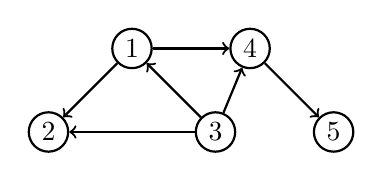
\begin{tikzpicture}[auto,node distance=1.5cm,
        thick,main node/.style={circle,draw,minimum size=0.5cm,inner sep=0pt]}]

    \node[main node] (1) {$1$};
    \node[main node] (2) [below left of=1]  {$2$};
    \node[main node] (3) [below right of=1] {$3$};
    \node[main node] (4) [right of=1] {$4$};
    \node[main node] (5) [right of=3] {$5$};

    \path[->]
    (1) edge node {} (2)
        edge node {} (4)
    (3) edge node {} (1)
        edge node {} (2)
        edge node {} (4)
    (4) edge node {} (5);
\end{tikzpicture}
\\\centering A graph $G = (V, E, w)$. 
\end{minipage}
\begin{minipage}[b]{0.33333\textwidth}
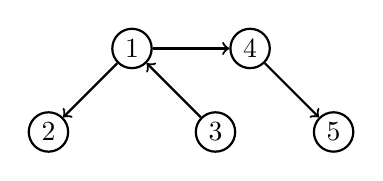
\begin{tikzpicture}[auto,node distance=1.5cm,
        thick,main node/.style={circle,draw,minimum size=0.5cm,inner sep=0pt]}]

    \node[main node] (1) {$1$};
    \node[main node] (2) [below left of=1]  {$2$};
    \node[main node] (3) [below right of=1] {$3$};
    \node[main node] (4) [right of=1] {$4$};
    \node[main node] (5) [right of=3] {$5$};

    \path[->]
    (1) edge node {} (2)
        edge node {} (4)
    (3) edge node {} (1)
    (4) edge node {} (5);
\end{tikzpicture}
\\\centering A spanning tree of $G$. 
\end{minipage}
\begin{minipage}[b]{0.33333\textwidth}
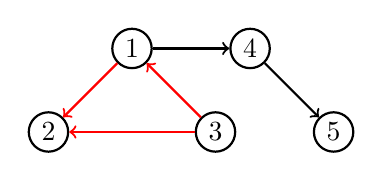
\begin{tikzpicture}[auto,node distance=1.5cm,
        thick,main node/.style={circle,draw,minimum size=0.5cm,inner sep=0pt]}]

    \node[main node] (1) {$1$};
    \node[main node] (2) [below left of=1]  {$2$};
    \node[main node] (3) [below right of=1] {$3$};
    \node[main node] (4) [right of=1] {$4$};
    \node[main node] (5) [right of=3] {$5$};
s
    \path[->]
    (1) edge node {} (4)
    (4) edge node {} (5);
    \path[->, red]
    (3) edge node {} (1)
    (1) edge node {} (2)
    (3) edge node {} (2);
    
\end{tikzpicture}
\\\centering Edge $(3,2)$'s cycle, shown in red. 
\end{minipage}
\caption{An example graph and spanning tree with off-tree edges $(3,2)$ and $(3,4)$}
\label{ex:cycle}
\end{figure}
\begin{definition}(Tree Path)
    For $a,b \in V$, the tree path $P_{(a,b)} \subseteq V \times V$ is the unique path between $a$ and $b$ in $T$.
\end{definition}
\begin{definition}(Tree Cycle)
    For $a,b \in V$, the tree cycle $C_{(a,b)} = \{(a,b)\} \cup P_{(a,b)}$. The vector $\vec c_{(a,b)} \in \R^E$ assigns flow $1$ to each edge $e \in C_{(a,b)}$. 
\end{definition}

\noindent A path $P_e$ corresponds to a vector $\vec p_e$ as follows: for $a,b \in V$, $$\vec p_{e}((a,b)) = \begin{cases} 1 & (a,b) \in P_{e} \cap E \\ -1 & (a,b)  \in P_{e} \land (b,a) \in E  \\ 0 & \text{o.w.} \end{cases}$$

A cycle $C_e$ corresponds to a  vector $\vec c_e$, which is defined analogously to $\vec p_e$. The vector corresponding to a cycle is a circulation, which, recall, means that $B^T \vec c_e = 0$. 


The set of all circulations $\{ \vec c \in \R^E : B^T\vec c = 0\}$ is a subspace called the \textit{cycle space} and the cycles $\{ \vec c_e : e \in E \setminus E_T \}$  determined by the off-tree edges are a basis for this space. 

\begin{example}
    Continuing the example of Figure \ref{ex:cycle}, the cycle basis is $\{ \vec c_{(3,2)}, \vec c_{(3,4)} \}$. The cycle $C'$ with path $\{ (3,2), (2,1), (1,4), (4,3) \}$ and vector $\vec c'$ is not in this basis, but it can be formed from basis elements.
    \begin{figure}[H]
    \begin{minipage}{0.48\textwidth}
    \centering 
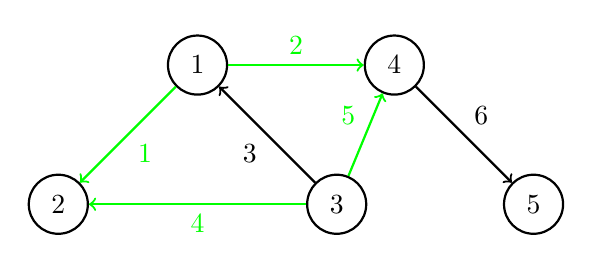
\begin{tikzpicture}[auto,node distance=2.5cm,
        thick,main node/.style={circle,draw,minimum size=0.75cm,inner sep=0pt]}]

    \node[main node] (1) {$1$};
    \node[main node] (2) [below left of=1]  {$2$};
    \node[main node] (3) [below right of=1] {$3$};
    \node[main node] (4) [right of=1] {$4$};
    \node[main node] (5) [right of=3] {$5$};

    \path[->]
    (3) edge node {3} (1)
    (4) edge node {6} (5);
    \path[->, green]
    (1) edge node {1} (2)
        edge node {2} (4)
    (3) edge node {4} (2)
    (3) edge node {5} (4);
\end{tikzpicture}
\\\centering 
\end{minipage}
\begin{minipage}{0.48\textwidth}
\vspace{-10px}
    $$\textcolor{red}{\vec c_{(3,2)}} = 
    \textcolor{red}{
    \begin{bmatrix}
        -1 \\ 0 \\ -1 \\ 1 \\ 0 \\ 0 
    \end{bmatrix}}, \vec c_{(3,4)} = \begin{bmatrix}
        0 \\ -1 \\ -1 \\ 0 \\ 1 \\ 0 
    \end{bmatrix},
    \textcolor{green}{\vec c'} = \textcolor{green}{\begin{bmatrix}
        -1 \\ 1 \\ 0 \\ 1 \\ -1 \\ 0 
    \end{bmatrix}} = \textcolor{red}{\vec c_{(3,2)}} - \vec c_{(3,4)}
    $$
\end{minipage}
\caption{The composite cycle $C'$, shown in green, is comprised of  basis cycles. }
\end{figure}
\end{example}

A given graph may have several spanning trees, some of which result in faster convergence of the algorithm than others. We quantify the desirability of a spanning tree according to its \textit{condition number}. This number represents how well the resistances of off-tree edges are approximated by the resistance along the cycle determined by that edge. 
\begin{definition}[Cycle Resistance $R_e$]$R_e = \sum_{e' \in C_e} r_{e'} = \vec c_e^T R \vec c_e$
\end{definition}
\begin{definition}[Tree Condition Number $\tau$]
    $\tau(T) = \sum_{e\ in E \setminus E_T} \frac{R_e}{r_e}$. 
\end{definition}
\begin{definition}[Stretch $st$] For $e \in E$, $st(e) = \frac{\sum_{e' \in P_e} r_{e'}}{r_e}$ and $st(T) = \sum_{e \in E} st(e)$.
\\
\\
We remark that $\tau(T) =  st(T) + m - 2n + 2 $; so, a low-stretch tree has a low condition number. Other works have yielded useful techniques for producing low-stretch spanning trees. 

\begin{theorem}[\cite{AN12}] 
\label{thm:AN12}
    In $\mathcal O(m \log n \log \log n)$ time we can compute a spanning tree $T$ with a total stretch $st(T) = O(m \log n \log \log n)$. 
\end{theorem}
    
\end{definition}



% Generally speaking, given an inner product $\langle ., . \rangle$, the orthogonal projection of $x$ along $y$ (resp. $y^\perp$) in that inner product space is $Proj_y(x) = \frac{\langle y, x \rangle }{ \langle y , y\rangle}y$ (resp. $Proj_{y^\perp}(x) = x - \frac{\langle y, x \rangle}{ \langle y , y\rangle}y$). Noting that $\langle \vec a , \vec b \rangle = \vec a^T R\vec b$ is an inner product, denote $S$ this inner product space. Since $\| \vec a \|^2_R = \langle \vec a, \vec a \rangle$, we can see that the above expression $\vec f_i - \frac{\vec f_i^T R \vec c_{e_i}  }{\| \vec c_{e_i}\|^2_R} c_{e_i}$ is an orthogonal projection of $\vec f_i$ along $\vec c_{e_i}^\perp$ in $S$, in the ordinary sense of projection, meaning that this projection operator $\Pi_{e_i}$ is symmetric and idempotent. 